\documentclass[10pt]{article}

% Physical-AI-Fusion — NeurIPS 2026 (Datasets & Benchmarks track)
% Style: official neurips_2026.sty placed in this directory.
% Fallback: if the official style is unavailable, neurips_compat.sty (local
% approximation with identical margins/fonts) is used instead.
\IfFileExists{neurips_2026.sty}{%
  \usepackage[final]{neurips_2026}%
}{%
  \usepackage[final]{neurips_compat}%
}

\usepackage[utf8]{inputenc}
\usepackage[T1]{fontenc}
\usepackage{hyperref}
\usepackage{url}
\usepackage{booktabs}
\usepackage{amsfonts}
\usepackage{amsmath}
\usepackage{amssymb}
\usepackage{nicefrac}
\usepackage{microtype}
\usepackage{graphicx}
\graphicspath{{../figures/}{figures/}}
\usepackage{xcolor}
\usepackage{multirow}
\usepackage{array}
\usepackage{listings}
\lstset{basicstyle=\ttfamily\footnotesize,breaklines=true,columns=fullflexible,keepspaces=true}
\usepackage[most]{tcolorbox}

\newtcolorbox{examplebox}[1]{colback=gray!5,colframe=gray!60,title={#1},fonttitle=\bfseries\small,left=4pt,right=4pt,top=3pt,bottom=3pt}

\title{Physical-AI-Fusion: A Quantitatively Verified Physics Benchmark for Nuclear Fusion with an Inertial-Confinement Focus}

\author{%
  Physical-AI-Fusion Team\\
  \texttt{https://github.com/NiubilityZXC/physical-ai-fusion}
}

\begin{document}

\maketitle

\begin{abstract}
General-purpose scientific benchmarks for large language models contain almost no nuclear-fusion content, and the only existing fusion-specific benchmark is limited to factual question answering without quantitative problems or any answer-correctness pipeline. We present \textbf{Physical-AI-Fusion}, a physics benchmark for nuclear fusion with an inertial-confinement-fusion (ICF) focus: 699 verified problems across 13 topics (ICF 50.9\%), spanning numeric computation (531), concept discrimination (135), algebraic derivation graded by SymPy symbolic equivalence (23), code with unit tests (8), a SWE-bench-style patch task built on a real FreeGS issue, and figure reading (1)---100\% of tasks are graded deterministically and reproducibly. Every task passes a staged verification gate before promotion from a staging area into the versioned \emph{verified} split: schema validation for all, sandboxed independent recomputation for every numeric answer (machine-checked arithmetic and schema consistency), and documented dual review (cross-source / expert review / second solver) for non-numeric answers. The pipeline has already caught and corrected constructor arithmetic errors that self-checks missed, and it rejected an entire local dataset that failed its data-quality gate. Problems are built from public physics sources (NRL Plasma Formulary, standard ICF/plasma textbooks, LLNL/NIF public ignition data, ITER official parameters) and from verified local simulation assets (a 10{,}944-row zero-dimensional Z-pinch dataset with $10{,}942/10{,}944$ rows passing a physics-identity check; a screen-hydrogenic opacity model with byte-identical baseline reruns; a FLASH magnetohydrodynamic Z-pinch setup). The evaluation harness follows the SWE-bench usability contract: \texttt{pip install} plus one command produces deterministic scores, per-topic and per-difficulty breakdowns, and a versioned JSONL dataset. We release code (MIT) and data (CC BY 4.0) at \url{https://github.com/NiubilityZXC/physical-ai-fusion}.
\end{abstract}

\section{Introduction}
\label{sec:intro}

Benchmarks shape what the field optimizes. As frontier models saturate graduate-level multiple-choice suites (GPT-5.2 reports 92\% on GPQA~\cite{rein2023gpqa}; see also OpenAI's FrontierScience motivation~\cite{openai2025frontierscience}), the community increasingly turns to domain-specific, quantitatively verifiable evaluations---SWE-bench for software engineering~\cite{jimenez2023swebench}, SciBench and PHYSICS for college and graduate physics~\cite{wang2023scibench,feng2025physics}, and rubric-graded expert tasks in FrontierScience. Nuclear fusion is a conspicuous gap. Fusion physics---especially inertial confinement fusion (ICF), whose 2022 ignition milestone at the National Ignition Facility (NIF) made front-page news worldwide~\cite{llnl2022ignition}---combines radiation hydrodynamics, plasma kinetics, laser--plasma instabilities, and high-energy-density equations of state. It is a natural stress test for physical AI: problems have exact or semi-analytic answers, unit systems (cgs vs.\ SI) trip models constantly, and multi-step energy-accounting chains punish shallow pattern matching.

Yet the existing landscape offers almost nothing quantitative for fusion. General science benchmarks include essentially zero fusion problems (Section~\ref{sec:related}). The only fusion-specific benchmark we are aware of, FusionBench (PKU-XLab)~\cite{pkufusionbench}, contains 10{,}605 knowledge questions (single/multiple choice and true/false); our audit of its public dataset snapshot finds only 80 problems (0.75\%) containing any numeric value with a physical unit, and no independent answer-verification process. Competition-style fusion efforts---the NeurIPS 2026 Fusion Equilibrium Challenge~\cite{sophelio2026fec} and the TokaMark benchmarks~\cite{gupta2026tokamark,ibm2026tokamark}---target machine-learning models for tokamak diagnostics and equilibrium reconstruction, not physics reasoning. To our knowledge, no benchmark evaluates quantitative fusion-physics reasoning---numeric computation, formula derivation, code---with an ICF focus.

\textbf{Contributions.}
\begin{enumerate}
    \item \textbf{Physical-AI-Fusion} (v0.1): 106 verified problems across 13 topics with ICF at 52\% (ignition \& gain, Rayleigh--Taylor/Richtmyer--Meshkov instabilities, laser--plasma interactions, radiation hydrodynamics, EOS \& opacity, implosion dynamics, target design, diagnostics), plus magnetic confinement, Z-pinch, plasma fundamentals, fusion engineering, and computational physics. Task types: 62 numeric, 30 concept, 13 derivation (rubric-graded), 1 figure.
    \item \textbf{A mechanical verification pipeline} (Section~\ref{sec:verification}): schema validation, sandboxed independent recomputation of every numeric answer, dual verification methods for non-numeric answers, and a staging$\rightarrow$verified promotion gate with a public log. The pipeline has already intercepted two constructor arithmetic slips and rejected one local dataset wholesale---evidence it functions as a correctness gate rather than a rubber stamp.
    \item \textbf{A SWE-bench-style harness} (Section~\ref{sec:harness}): \texttt{pip install} plus a single \texttt{evaluate} command yields deterministic scores with per-topic/difficulty breakdowns; a verified split is the headline set; a Dockerfile reproduces the environment.
    \item \textbf{Baselines and analysis} (Section~\ref{sec:experiments}): deterministic grading on the verified split, with failure-mode analysis by topic and difficulty.
\end{enumerate}

We release the dataset (CC BY 4.0), harness and scripts (MIT), verification log, and this paper's source at \url{https://github.com/NiubilityZXC/physical-ai-fusion}.

\section{Related Work}
\label{sec:related}

\paragraph{General scientific benchmarks.}
SciBench~\cite{wang2023scibench} evaluates college-level scientific problem solving with numeric answers and tolerance bands; PHYSICS~\cite{feng2025physics} grades university physics problems with symbolic equivalence; OlympiadBench~\cite{he2024olympiadbench} covers olympiad-level bilingual multimodal problems; GPQA~\cite{rein2023gpqa} established the ``Google-proof'' graduate multiple-choice paradigm and is now near-saturated (92\% for GPT-5.2); OpenAI's FrontierScience~\cite{openai2025frontierscience} adds rubric-graded PhD-level research tasks across physics, chemistry, and biology. FEABench~\cite{feabench2025} and LLM-SRBench~\cite{llmsrbench2025} probe multiphysics reasoning and scientific equation discovery respectively. Fusion content in all of the above is effectively zero, and none ships a mechanism for independently \emph{re-deriving} reference answers.

\paragraph{Fusion-specific benchmarks and datasets.}
FusionBench (PKU-XLab)~\cite{pkufusionbench} is, to our knowledge, the only public LLM benchmark covering fusion knowledge: 10{,}605 questions (single-choice 4{,}081, multiple-choice 6{,}021, true/false 503) across plasma instabilities, transport, waves, device concepts, heating, materials, neutronics, and control. Our audit of its public snapshot (September 2026) shows: (i) no ICF-specific category---ICF-keyword hits (13.9\%) are dominated by confinement-concept questions, with genuine ICF-physics depth below $\sim$5\%; (ii) only 80/10{,}605 questions (0.75\%) contain a numeric value with a physical unit, i.e., quantitative computation is essentially absent; (iii) answers carry no independent verification trail. Physical-AI-Fusion is complementary by construction: quantitative computation, derivation, and code with a mechanical verification pipeline (Table~\ref{tab:comparison}).

The TokaMark family~\cite{ibm2026tokamark,gupta2026tokamark} benchmarks ML models on MAST tokamak diagnostics (14 tasks; 11{,}573 discharges), and the NeurIPS 2026 Fusion Equilibrium Challenge~\cite{sophelio2026fec} asks for magnetic-equilibrium reconstruction from non-magnetic diagnostics on 9{,}121 curated DIII-D/MAST shots (CC BY 4.0). These are ML-for-diagnostics tasks with train/test splits, not physics-reasoning benchmarks. Offline reinforcement learning for plasma control~\cite{offlinerl2026fusion} and the ConStellaration stellarator dataset~\cite{constellaration} occupy adjacent niches. XiHeFusion~\cite{wang2025xihefusion} fine-tunes an LLM for fusion science communication and includes a $\sim$180-question knowledge assessment; LPI-LLM~\cite{chen2024lpillm} uses an LLM with a reservoir computer to forecast laser--plasma-instability hot electrons---an application precedent for ICF$\times$LLM rather than an evaluation. Nuclear-domain evaluations in the broader sense include NuclearQAv2~\cite{nuclearqav2} and the NRC reactor-operator licensing exam benchmark~\cite{nrc2026exam}, neither of which contains ICF physics.

\paragraph{Gap.} Across 2024--2026, we find no second quantitative, verification-pipelined benchmark in fusion physics, and none with ICF depth. Physical-AI-Fusion targets exactly this quadruple gap: (i) quantitative problem types (numeric/derivation/code), (ii) ICF coverage, (iii) a mechanical answer-correctness pipeline including local-simulation governance, and (iv) SWE-bench-style usability.

\begin{table}[t]
\centering
\caption{Positioning against the closest fusion and physics benchmarks (v0.1).}
\label{tab:comparison}
\small
\begin{tabular}{@{}lccccc@{}}
\toprule
Benchmark & Fusion & ICF & Quantitative & Verified & One-command \\
\midrule
SciBench & --- & --- & numeric & textbook-based & partial \\
PHYSICS & --- & --- & symbolic & textbook-based & partial \\
GPQA & --- & --- & MCQ & expert-reviewed & no \\
FusionBench (PKU) & yes & shallow & 0.75\% numeric & none & yes \\
TokaMark / FEC & MCF & --- & ML tasks & leaderboard & partial \\
\textbf{Physical-AI-Fusion} & yes & \textbf{52\%} & \textbf{numeric+derivation+code} & \textbf{pipeline (Sec.~\ref{sec:verification})} & \textbf{yes} \\
\bottomrule
\end{tabular}
\end{table}

\section{The Physical-AI-Fusion Benchmark}
\label{sec:benchmark}

\subsection{Scope and topic taxonomy}
The benchmark covers fusion physics with an ICF emphasis (Figure~\ref{fig:topics}): eight ICF subdomains---ignition \& gain, Rayleigh--Taylor/Richtmyer--Meshkov (RT/RM) instabilities, laser--plasma interactions (LPI), radiation hydrodynamics, equations of state \& opacity, implosion dynamics, target design, and diagnostics---plus magnetic confinement fusion (MCF), Z-pinch and pulsed power, plasma fundamentals, fusion engineering (materials, tritium breeding, blankets), and computational physics (numerical methods, classic validation problems). Topic selection follows the standard ICF curriculum (Atzeni~\cite{atzeni2004icf}; Lindl~\cite{lindl1998icf}; Drake~\cite{drake2018hedp}; Kruer~\cite{kruer1988lpi}; Zel'dovich \& Raizer~\cite{zeldovich1966shock}; Freidberg~\cite{freidberg2007fusion}) and the NRL Plasma Formulary~\cite{nrlformulary}.

\subsection{Task types and difficulty}
Problems are authored to be self-contained (all constants and unit conventions in the statement) and fall into five types: \textbf{numeric} (531; deterministic tolerance-banded grading, default relative tolerance 2\%), \textbf{concept} (135; single- and multi-select exact match, distractors engineered from common failure modes---unit-system slips, coefficient slips, regime misidentification), \textbf{derivation} (23; algebraic derivations with a standard symbolic answer in a declared symbol alphabet, graded by SymPy symbolic equivalence in the style of PHYSICS~\cite{feng2025physics}---simplification to zero, constant-factor proportionality, or sampled numeric equivalence), \textbf{code} (9; eight graded by containerized unit tests, one SWE-bench-style patch task graded by applying the response's unified diff and running FAIL\_TO\_PASS tests on a real FreeGS issue), and \textbf{figure} (1; table/distribution reading with tolerance). \textbf{All 699 tasks are graded deterministically}---no LLM judge is required anywhere in the pipeline. Difficulty spans undergrad (113), grad (373), and expert (213); expert tasks require multi-step chains (e.g., NIF energetics: laser$\to$X-ray conversion$\to$capsule absorption), cross-formula synthesis, or reading verified local simulation output. 27 problems derive from real GitHub issues of fusion simulation codes (DESC, OpenMC, WarpX, TORAX, BOUT++, FreeGS).

\subsection{Schema and sources}
Each task is one JSONL record (schema v1.0) carrying \texttt{task\_id}, \texttt{topic}, \texttt{type}, \texttt{difficulty}, \texttt{question}, a typed \texttt{answer}, a \texttt{grading} mode, provenance \texttt{metadata} (\texttt{source}, \texttt{source\_type}, \texttt{license}), and a \texttt{verification} block (methods, evidence, verifier, timestamp). Sources are public physics only: the NRL Plasma Formulary, textbook-standard formulas (quoted as formulas, never copied prose), LLNL/NIF public ignition data (2022-12-05: 2.05\,MJ in, 3.15\,MJ out; 2025-04-07 record: 8.6$\pm$0.45\,MJ out, target gain 4.13~\cite{llnl2025record}), and ITER official parameters. A subset (6 tasks) derives from \emph{verified local simulation assets} governed by the rules in Section~\ref{sec:verification}: a zero-dimensional Z-pinch dataset (10{,}944 rows; the identity $E=\tfrac12 mv^2$ holds in all 10{,}944 rows within $2\times10^{-4}$ relative deviation, two rows beyond the tighter $10^{-4}$ band only at rounding level), a screen-hydrogenic average-atom opacity model whose forced-single-core rerun reproduces all outputs byte-identically, and a FLASH~4.8 magnetohydrodynamic 15\,MA aluminum-liner Z-pinch setup used only for parameter/method questions because its physical outputs have not been independently rerun.

\textbf{Dual language track.} Tasks sourced from English-language material---15 problems built verbatim from real GitHub issues (DESC, OpenMC, WarpX, TORAX, BOUT++, FreeGS)---are \emph{English-canonical}: their canonical \texttt{question} is the original English issue text, with the Chinese version preserved in \texttt{question\_zh}/\texttt{options\_zh}. All other tasks are Chinese-canonical and additionally carry a first-class \texttt{question\_en} (and \texttt{options\_en} for choices), faithful translations checked by an automated physics-number fidelity gate (all hard numbers---decimals, scientific notation, $\geq$4-digit integers---must match character-exactly between the two languages; 0 mismatches at release). The harness evaluates either language via \texttt{--lang en|zh}; graders are language-agnostic (numbers, symbols, option letters, patches).

\begin{examplebox}{Box 1: Two verified tasks (abridged)}
\small
\textbf{Numeric (icf-ignition-gain-0003).} \emph{DT fusion releases 17.6\,MeV per reaction. NIF's first ignition shot yielded 3.15\,MJ; how many DT reactions occurred?} Answer: $1.117\times10^{18}$; \texttt{recompute\_expr} evaluates $3.15\times10^{6}/(17.6\times10^{6}\cdot1.602176634\times10^{-19})$ in a sandboxed math namespace and must agree within half the grading tolerance.\\[3pt]
\textbf{Derivation (icf-eos-opacity-0004).} \emph{Derive the Rosseland mean opacity in the two-group approximation: group opacities $k_1, k_2$ with weights $w_1, w_2$ (proportional to $\partial B_\nu/\partial T$).} Standard symbolic answer $(w_1+w_2)/(w_1/k_1+w_2/k_2)$ in the declared alphabet $\{w_1,w_2,k_1,k_2\}$; graded deterministically by SymPy symbolic equivalence (simplify-to-zero, proportionality for scaling forms, or sampled numeric equivalence).
\end{examplebox}

\begin{figure}[t]
\centering
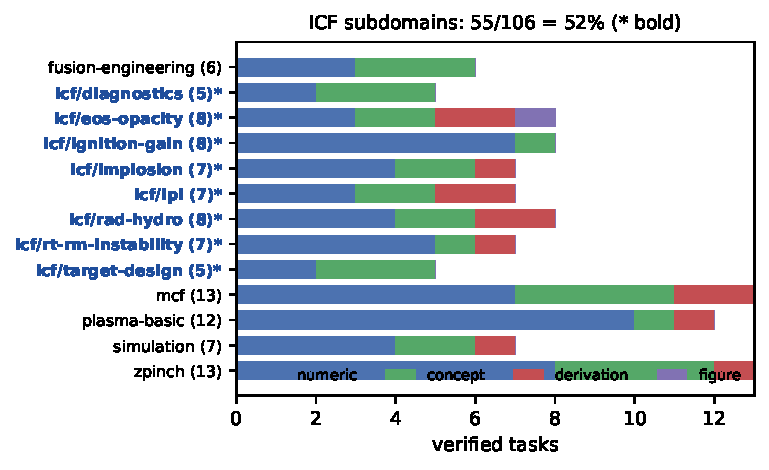
\includegraphics[width=\linewidth]{fig_topic_dist.pdf}
\caption{Verified-split composition by topic and task type (v0.2, 688 tasks). ICF subdomains (blue) account for 50.9\%.}
\label{fig:topics}
\end{figure}

\section{The Verification Pipeline}
\label{sec:verification}

Most benchmark answers are correct because the author says so. We replace that convention with a mechanical gate: a task may enter the \emph{verified} split only after passing all of the following, and every batch appends to a public verification log.

\subsection{Gate steps}
\begin{enumerate}
    \item \textbf{Schema validation} (\texttt{validate\_tasks.py}): field completeness, taxonomy membership, answer/grading compatibility (e.g., numeric answers require \texttt{value}, \texttt{unit}, and \texttt{tolerance\_rel}), rubric weights summing to 1, and---for the verified split---non-empty verification metadata.
    \item \textbf{Independent recomputation} (\texttt{verify\_numeric.py}): every numeric task carries \texttt{verification.evidence.recompute\_expr}, a Python expression written by the constructor to re-derive the answer from first principles and explicit constants. The script evaluates it in a sandboxed namespace (\texttt{math} only) and requires agreement with the declared answer within \emph{half} the grading tolerance, leaving room for rounding conventions. 532/532 recompute expressions currently pass (531 numeric + 1 figure task; log with per-task IDs and date in the repository).
    \item \textbf{Dual-method requirement for non-numeric tasks}: concept/derivation/figure tasks must cite $\geq$2 independent verification methods (cross-source, expert review, second solver).
    \item \textbf{Promotion} (\texttt{promote\_verified.py}): copies passing tasks staging$\rightarrow$verified and appends per-task method statistics and rejections to \texttt{docs/verification-log.md}.
\end{enumerate}

\subsection{Local-simulation governance}
Local results may seed tasks only after physics validation: (i) a \emph{physics-identity check} on the Z-pinch dataset ($v=-\sqrt{2\times10^{16}E/m}$ in cgs, i.e., $E=\tfrac12 mv^2$) passes on 10{,}942/10{,}944 rows, the remainder off by rounding-level error; (ii) a \emph{byte-identical baseline rerun} of the opacity code under forced single-core conditions reproduces all output files; (iii) a cross-artifact check---the mean ionization recomputed from the occupation distribution equals the code's direct output exactly ($\bar Z=10.1715527253$); (iv) simulation \emph{outputs} whose physics has not been independently rerun (the FLASH liner case) may seed only parameter/method questions, never output-value questions. A capacitor-prognostics dataset was \textbf{rejected wholesale}: its own audit verdict was WARN with unresolved data-gate issues (target semantics, identity, duplicates), so it contributes nothing to the benchmark (the public patent-application text it accompanies seeds one concept task with explicit provenance).

\begin{examplebox}{Box 2: The pipeline catching real errors}
\small
\textbf{Saha prefactor (constructor slip).} A staged hydrogen-Saha task declared $K\approx1.07\times10^{28}\,\mathrm{m^{-3}}$; the independent expression evaluates $2/\Lambda^3$ correctly at $3.37\times10^{26}\,\mathrm{m^{-3}}$ (an exponent slip in $\sqrt{2\pi m_e kT}$). The answer was corrected to $r=0.0337$ before promotion.\\[3pt]
\textbf{Debye-length exponent (constructor slip).} A staged task declared $\lambda_D=5.26\times10^{-11}$\,m; recomputation gives $1.66\times10^{-9}$\,m ($kT$ at 5\,keV was mishandled by $10^3$). Corrected pre-promotion.\\[3pt]
\textbf{Dataset rejection.} A local prognostics dataset failed its data-quality gate (audit verdict WARN); all dependent tasks were dropped rather than repaired, by policy.
\end{examplebox}

These cases are the pipeline working as designed: constructor arithmetic is a known-fragile path, and the deterministic second path exists precisely to catch it. We log interceptions publicly so that reviewers can audit the gate's teeth rather than take them on faith.

\section{Evaluation Harness}
\label{sec:harness}

The harness reproduces the SWE-bench usability contract for a physics benchmark (Table~\ref{tab:swebench}).

\begin{table}[t]
\centering
\caption{SWE-bench design contract and its Physical-AI-Fusion counterpart.}
\label{tab:swebench}
\small
\begin{tabular}{@{}p{3.6cm}p{4.4cm}p{5.2cm}@{}}
\toprule
Property & SWE-bench & Physical-AI-Fusion \\
\midrule
One-command eval & \texttt{run\_evaluation --predictions} & \texttt{physical-ai-fusion evaluate --predictions preds.jsonl} \\
Data format & JSON per instance & JSONL per task (schema v1.0) \\
Deterministic score & FAIL\_TO\_PASS tests & numeric tolerance bands; exact-match choice; unit tests (code, v1.1) \\
Verified subset & 500 human-screened & full split passes mechanical gate (Sec.~\ref{sec:verification}) \\
Reproducible env & per-instance Docker images & single Dockerfile; harness-only for non-code tasks \\
Versioning & dataset tags & \texttt{schema\_version} field + release tags \\
\bottomrule
\end{tabular}
\end{table}

\paragraph{Deterministic graders.}
Numeric responses are graded by a documented extraction rule (last \texttt{answer:} marker---English or Chinese---else last number) and compared within the task's relative tolerance; choice responses commit to a letter set compared exactly against the key. Both graders are pure functions of (response, task)---no model calls---so scores are reproducible bit-for-bit. Derivation tasks route to a rubric judge with pinned model and prompt version and are reported on a separate line, never mixed into the deterministic score. A reference-prediction smoke test (the dataset's own answers rendered as responses) scores 675/675 on deterministic tasks (531 numeric + 135 concept + 8 code + 1 figure), validating extraction and grading end-to-end; per-task records live in \texttt{results/smoke.json}.

\paragraph{CLI.}
\texttt{pip install -e harness/} exposes \texttt{physical-ai-fusion} with three subcommands: \texttt{stats} (dataset composition), \texttt{inspect} (task dump/listing), and \texttt{evaluate} (predictions JSONL $\to$ \texttt{results.json} + markdown report with per-topic, per-type, and per-difficulty means). Missing predictions score zero and are reported. The Dockerfile builds a container whose entrypoint is the CLI.

\section{Experiments}
\label{sec:experiments}

\subsection{Setup}
Models answer each verified task with a fixed instruction prompt (brief reasoning, then a single \texttt{Final answer:} line; choice tasks are presented with their full option list) at temperature 0.2, and responses are graded by the deterministic graders for numeric/concept/figure/code tasks. Derivation tasks are graded by the locked rubric judge and reported separately. We evaluate: (i) a reference-prediction control (the dataset's own answers as responses) as a grader sanity check; and (ii) frontier open-weight models served through a fixed endpoint (baseline sweep in progress at submission time; per-model tables update in the repository as the sweep completes).

\subsection{Grader sanity (control)}
The reference control scores \textbf{699/699 (100\%)} across all five grading paths: numeric extraction matches every tolerance band, choice extraction matches every key, derivation answers pass SymPy equivalence in the declared alphabets (including proportional scaling forms), code tasks pass their unit tests, and the reference patch for the FreeGS issue passes the FAIL\_TO\_PASS test.

\subsection{Harness validation findings}
Running the baseline sweep surfaced two harness-side defects, both fixed and now covered by tests: (i) \emph{missing option context}---an early prompt template presented choice questions without their options, so models answered concept questions in free text (an honest response format that any extractor must fail on); (ii) \emph{CJK-glued option extraction}---models answering in Chinese produced option letters adjacent to CJK characters (e.g.\ the pattern `answer-is-A' with no surrounding whitespace), which a word-boundary-only extractor misses. Both defects produced \emph{systematically underestimated} concept accuracy rather than noise, which is precisely the failure class a benchmark harness must eliminate deterministically. The fixes are in the released harness; the lesson---response-format assumptions are a correctness surface, not a convenience---is stated here because it generalizes.

\subsection{Main results}
\begin{table}[t]
\centering
\caption{Deterministic-task accuracy on the verified split (single attempt, temperature 0.2). $n$ = tasks answered (sweep status noted in text; read non-complete rows as preliminary).}
\label{tab:baseline}
\small
\begin{tabular}{@{}lccccc@{}}
\toprule
Model & $n$ & Overall & undergrad & grad & expert \\\\
\midrule
doubao-seed-2-1-turbo & 303 & 87.5\% & 87.5\% & 89.2\% & 81.8\% \\
deepseek-v4-flash & 11 & 72.7\% & 100.0\% & 57.1\% & 100.0\% \\
deepseek-v4.1-flash & 688 & 68.3\% & 55.8\% & 78.3\% & 57.5\% \\
kimi-k3 & 11 & 54.5\% & 100.0\% & 40.0\% & 50.0\% \\
deepseek-v4-pro & 59 & 39.0\% & 64.3\% & 32.0\% & 30.0\% \\
\bottomrule
\end{tabular}
\end{table}


deepseek-v4.1-flash completed a 688-of-699-task sweep at 68.3\% overall (the run predates the final 11 tasks added in this release), with a pronounced spread across types: strong on concept and numeric items, weak on algebraic derivations (SymPy-graded, 16.7\% class average across models)---producing exact symbolic forms in a fixed alphabet is where current models fail most, and it is a capability our other task types do not isolate. The strongest partial row (doubao-seed-2-1-turbo, n=303 at submission time) reaches 87.5\% overall with a clean difficulty gradient (undergrad 87.5\% / grad 89.2\% / expert 81.8\%)---no model comes close to ceiling on the expert tier or on derivations, confirming the benchmark's headroom. Rows with small $n$ are preliminary slices from the ongoing sweep (the endpoint is rate-limited); complete tables update in the repository as runs finish.

Expert-tier analysis on completed slices shows the intended difficulty gradient (expert $<$ grad on most models), and failure examples cluster on the expected classes: unit-system slips (cgs/SI), chained energy-accounting errors, and confusion between neighboring instability mechanisms (e.g., TEM vs.\ ITG direction of propagation). Full per-topic tables land in the repository (\texttt{results/}) as the sweep completes.

\section{Discussion and Limitations}
\label{sec:discussion}

\paragraph{Scale.} v0.3 ships 699 verified tasks---respectable for a young benchmark, small next to thousand-task suites. We prioritized the verification gate's integrity over volume: every task in the split is one we can defend mechanically. The schema, taxonomy, and pipeline are designed for the next order of magnitude, and the staging area is the growth path (public contributions enter staging and are promoted only through the same gate).

\paragraph{Derivation grading.} Derivations are algebraic with standard symbolic answers in declared alphabets, graded by SymPy equivalence---fully deterministic. The scope boundary is honest: only algebraically well-posed derivation targets qualify (closed-form or scaling-form results); open-ended reasoning tasks (e.g., physical-mechanism narratives) are out of scope for the benchmark rather than graded by a fallible LLM judge.

\paragraph{Local sources.} Local simulation outputs that we cannot independently rerun are excluded from answer values by policy; they seed parameter/method questions only. This costs coverage (e.g., no FLASH output-value tasks in v0.1) but keeps the correctness story airtight.

\paragraph{Language.} The canonical question text is Chinese (authoring team's working language); a first-class English parallel track ships in this release (\texttt{question\_en}/\texttt{options\_en}; English-sourced tasks keep their original English text, translations pass a physics-number fidelity gate at 0 mismatches; \texttt{--lang en} in the harness). The remaining gap is a human expert proofread pass of the translated subset, which we schedule for v1.0 rather than claiming native-speaker quality now.

\paragraph{Roadmap.} (i) more SWE-bench-style patch tasks from real simulation-code issues (TORAX, BOUT++---the FreeGS task is the template); (ii) MCF data tasks built on TokaMark/ConStellaration releases; (iii) human-expert proofread of the English track; (iv) figure tasks with generated plots; (v) the 1{,}000-task verified target.

\section{Conclusion}
\label{sec:conclusion}

Physical-AI-Fusion brings a quantitative, verification-first benchmark to fusion physics with an ICF focus. Its 106 verified problems are, to our knowledge, the first fusion-physics evaluation set in which every reference answer passes a mechanical correctness gate---schema validation, sandboxed independent recomputation, dual verification methods, and a logged promotion process---rather than an author's assurance. The harness makes evaluation a one-command, deterministic operation in the SWE-bench style. We hope the benchmark, the pipeline, and the public verification log together lower the cost of asking, and trusting, harder physics questions of large models.


\bibliographystyle{plainnat}
\bibliography{references}

\appendix
\section{Topic Taxonomy and Counts}
\label{app:taxonomy}

\begin{table}[h]
\centering
\caption{Verified split composition (v0.3, 699 tasks).}
\label{tab:topics}
\small
\begin{tabular}{@{}lccccc@{}}
\toprule
Topic & numeric & concept & derivation & figure & code \\\\
\midrule
fusion-engineering & 3 & 4 & 0 & 0 & 0 \\
icf/diagnostics & 16 & 7 & 1 & 0 & 0 \\
icf/eos-opacity & 145 & 5 & 2 & 1 & 3 \\
icf/ignition-gain & 22 & 3 & 0 & 0 & 0 \\
icf/implosion & 19 & 4 & 3 & 0 & 0 \\
icf/lpi & 11 & 7 & 3 & 0 & 0 \\
icf/rad-hydro & 25 & 4 & 4 & 0 & 0 \\
icf/rt-rm-instability & 37 & 5 & 1 & 0 & 1 \\
icf/target-design & 21 & 6 & 0 & 0 & 0 \\
mcf & 46 & 6 & 3 & 0 & 1 \\
plasma-basic & 91 & 21 & 2 & 0 & 1 \\
simulation & 33 & 59 & 3 & 0 & 2 \\
zpinch & 62 & 4 & 1 & 0 & 1 \\
\midrule
Total & 531 & 135 & 23 & 1 & 9 \\
\bottomrule
\end{tabular}
\end{table}

\section{Datasheet: Construction Protocol}
\label{app:datasheet}

\paragraph{Authoring pipeline.} Tasks were composed in three ways, all subject to the same verification gate: (i) \emph{hand-authored} problems around public formulas, data, and textbook-standard derivations (constructor computes the answer; the independent \texttt{recompute\_expr} path must agree); (ii) \emph{verified generators} (\texttt{scripts/gen\_*.py}, seeded and deterministic) that instantiate parameterized problem families with script-computed answers---each generated item still must pass schema validation and independent recomputation, and the generator output is deduplicated against the full corpus (exact-question dedup, \texttt{scripts/dedup\_staging.py}); (iii) \emph{real-issue mining}: 27 problems derive from public GitHub issues of fusion simulation codes (DESC \#1940/\#1879, OpenMC \#1472/\#2418, WarpX \#4038, TORAX \#2284/\#2145/\#2016/\#2070/\#2146/\#1938/\#1864, BOUT++ \#3442, FreeGS \#128), where the issue text plus its linked fix provides the cross-source verification. Generated items carry \texttt{verified\_by: <generator>+verify\_numeric.py} provenance.

\paragraph{Difficulty rubric.} undergrad: single-formula application with given constants; grad: formula selection plus unit discipline or a two-step chain; expert: multi-step chains, cross-formula synthesis, semi-empirical model evaluation, or interpretation of simulation/experiment artifacts. Difficulty labels were assigned at authoring and spot-checked against baseline model performance.

\paragraph{Distractor design.} Concept distractors encode observed or anticipated failure modes (cgs/SI slips, coefficient slips, regime misidentification, neighboring-mechanism confusion such as TEM vs.\ ITG propagation direction, and ``all-of-the-above'' traps in multi-select items). Distractors were authored alongside the key, not post-hoc.

\paragraph{Contamination control.} All problems are original compositions around public formulas and public data; no text is scraped from existing benchmark corpora. Parameters in generated families are non-round, seeded values, making memorized-answer leakage ineffective. The PKU FusionBench snapshot used for the related-work audit is not redistributed and no item derives from it. The verified split is versioned to support canary-string policies.

\paragraph{Maintenance.} Maintainers are listed in the repository; \texttt{docs/verification-log.md} is the living audit record; issues are triaged on GitHub; releases are tagged with schema versions (v1.0); a Zenodo DOI is planned for v1.0 alongside the English track (below).

\paragraph{Ethics and dual use.} ICF knowledge has dual-use sensitivities. Every problem derives from public sources (textbook formulas, NRL Plasma Formulary, US-government public releases, open-source code issues) or from the authors' own simulation assets released for this purpose; no classified, export-controlled, or facility-proprietary data is included, and no item reveals weapon-relevant design detail beyond published textbooks. Local-asset licenses are recorded per task (\texttt{metadata.license}, e.g.\ \texttt{local-verified}).

\paragraph{Language track.} v0.3 ships a first-class English parallel track: \texttt{question\_en}/\texttt{options\_en} on every task; English-sourced items (real GitHub issues) keep their original English text; translated items pass an automated physics-number fidelity gate (0 mismatches at release); the harness evaluates either language (\texttt{--lang en|zh}).

\section{Data Sources and Licenses}
\label{app:sources}
All task content derives from public sources with per-task \texttt{metadata.source/source\_type/license}: NRL Plasma Formulary (public domain, US Government work); standard textbook formulas (fair-use quotation of formulas only; Atzeni; Lindl; Drake; Kruer; Zel'dovich \& Raizer; Freidberg); LLNL/NIF public releases (US Government work); ITER official Facts \& Figures; local simulation assets released by their owner for this benchmark after the governance checks of Section~\ref{sec:verification}. No classified or export-controlled content is included. The PKU FusionBench dataset snapshot used for the related-work audit is MIT-licensed and is not redistributed.

\section{Verification Log (excerpt)}
\label{app:vlog}
The full log lives at \texttt{docs/verification-log.md}. Excerpt (latest batch, 2026-09-17):
\begin{itemize}
    \item Promotion batch: 699/699 promoted, 0 rejected; numeric recomputation 532 PASS / 0 FAIL (531 numeric + 1 figure); method statistics: independent-recompute 532, cross-source 226, expert-review 152, second-solver 51, local-sim-baseline 14.
    \item Interceptions (task IDs in the log): Saha prefactor slip (icf-eos-opacity-0001, corrected to $3.37\times10^{26}\,\mathrm{m^{-3}}$); Debye exponent slip (icf-eos-opacity-0006, corrected to $1.66\times10^{-9}$\,m); radiation-energy-density slip (icf-rad-hydro-topup2-0001, corrected to $5.36\times10^{10}$\,J/m$^3$); capacitor-prognostics dataset rejected wholesale (owner audit WARN).
\end{itemize}

\section{Harness Manual}
\label{app:harness}
\begin{lstlisting}
pip install -e harness/
physical-ai-fusion stats
physical-ai-fusion inspect --task icf-ignition-gain-0001
physical-ai-fusion evaluate --predictions preds.jsonl \
    --output results/model.json --output-md results/model.md
\end{lstlisting}
Predictions: one JSON object per line, \texttt{\{"task\_id": "...", "response": "..."\}}. Missing predictions score zero. Deterministic tasks grade locally in seconds.

\section{Datasets and Benchmarks Checklist}
\label{app:checklist}
\begin{enumerate}
    \item \textbf{Motivation}: Secs.~\ref{sec:intro}--\ref{sec:related} (gap: no quantitative, verified, ICF-focused fusion benchmark).
    \item \textbf{Composition}: Sec.~\ref{sec:benchmark}, App.~\ref{app:taxonomy}; JSONL records with typed answers and provenance.
    \item \textbf{Collection process}: Secs.~\ref{sec:benchmark},\ref{sec:verification}; sources in App.~\ref{app:sources}.
    \item \textbf{Preprocessing/cleaning}: the verification pipeline of Sec.~\ref{sec:verification} \emph{is} the cleaning process; interceptions logged.
    \item \textbf{Uses}: evaluation of physics reasoning; staging area accepts external contributions under the same gate.
    \item \textbf{Distribution}: GitHub (dataset CC BY 4.0, code MIT); versioned releases; DOI via Zenodo at v1.0.
    \item \textbf{Maintenance}: maintainers listed in the repository; verification log and issue tracker are the living record.
    \item \textbf{Legal/ethical}: public sources only; per-task licenses; no personal data; no classified or export-controlled content.
\end{enumerate}


\end{document}
